% DOC SETTINGS ===================================
\documentclass{article}
\usepackage[utf8]{inputenc}
\usepackage{steinmetz}
\usepackage{mathtools}  
\usepackage{multicol}
\usepackage{circuitikz}
\usepackage{tikz}
\usepackage{listings}
\usepackage{geometry}
\usepackage{fancyhdr}
\usepackage{amsfonts}
\usepackage{media9}
\usepackage{parskip}
\usetikzlibrary{positioning, fit, calc}
\pagestyle{fancy}
\lhead{ECE2804 Weekly Journal 3}
\rhead{Kavin Thirukonda 2021}
\fancyheadoffset{0mm}
 \geometry{
 a4paper,
 total={170mm,257mm},
 left=20mm,
 top=25mm,
 }
\mathtoolsset{showonlyrefs} 
\cfoot{}
% DOC SETTINGS ===================================
\begin{document}
\section*{Filter}
I first decided to completely redo the filter stage and simulate, build, and test it

first I figured out what the most important aspect to filter out was and determined it was to ensure that any high frequencies were filtered out. This was to protect against effects from the systems power supply. For this a low-pass filter must be implemented. 

I decided to go with a second order filter so that we could be sure any noise is gone and also get some gain. I decided on an $A_v$ gain of 1.5, and a cutoff frequency of $f_b = 3Hz$ which would get rid of unwanted parts of the AC signal.

Based on those values I can calculate the resistor values like so:
\begin{align}
    A_v &= 1.5 \\
    &= 1 + \frac{R_f}{R_i}\\
    Let\text{ }&R_f = 47k\Omega\\
    R_i &= \frac{R_f}{A_v-1}\\
    &= \frac{47k\Omega}{1.5-1}\\
    &= 94k\Omega
\end{align}
\begin{center}
    So, $\boxed{R_f = 47k\Omega}$ and $\boxed{R_i \cong 100k\Omega}$
\end{center}
\begin{align}
    f_b &= 3Hz \\
    &= \frac{1}{2\pi RC}\\
    Let\text{ }&C = 1\mu F\\
    R &= \frac{1}{2\pi f_bC}\\
    &= \frac{1}{2\pi \cdot3Hz \cdot 1\mu F}\\
    &= 53051.648\Omega
\end{align}
\begin{center}
    So, $\boxed{C = 1\mu F}$ and $\boxed{R\cong 56k\Omega}$
\end{center}
Now we can build the circuit in LTSpice:
\begin{center}
    \boxed{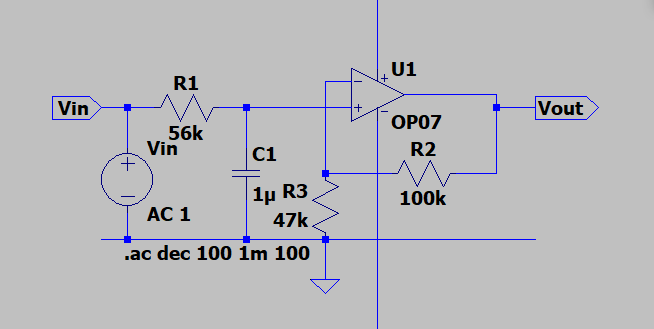
\includegraphics[width = .8\textwidth]{ltfilter.png}}
\end{center}
\textbf{All values were rounded to values available in the kit} so the simulation should be a good representation of the reality.
\newpage
Now by using LTSpice's analysis we get the bode plot of the circuit.
\begin{center}
    \boxed{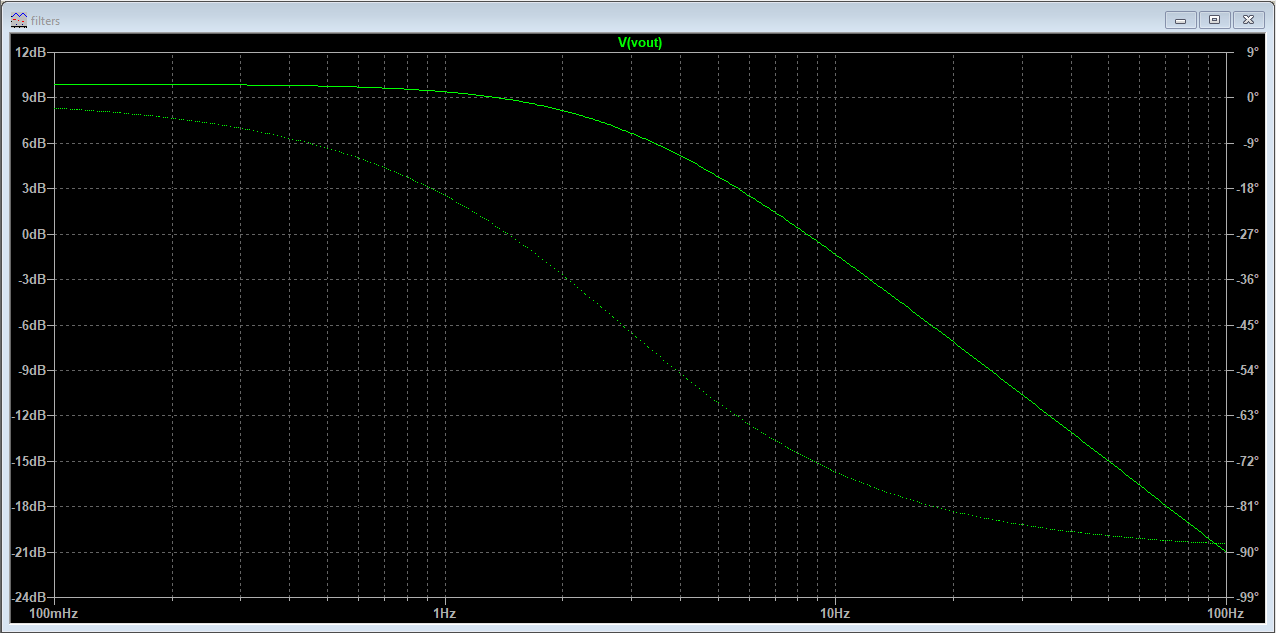
\includegraphics[width = .95\textwidth]{ltbode.png}}
\end{center}
As we can see the filter is serving its purpose and properly filtering out unwanted frequencies. Now that we know that the filter will serve our purpose we can build the circuit in real life and analyze it there.
\begin{center}
    \boxed{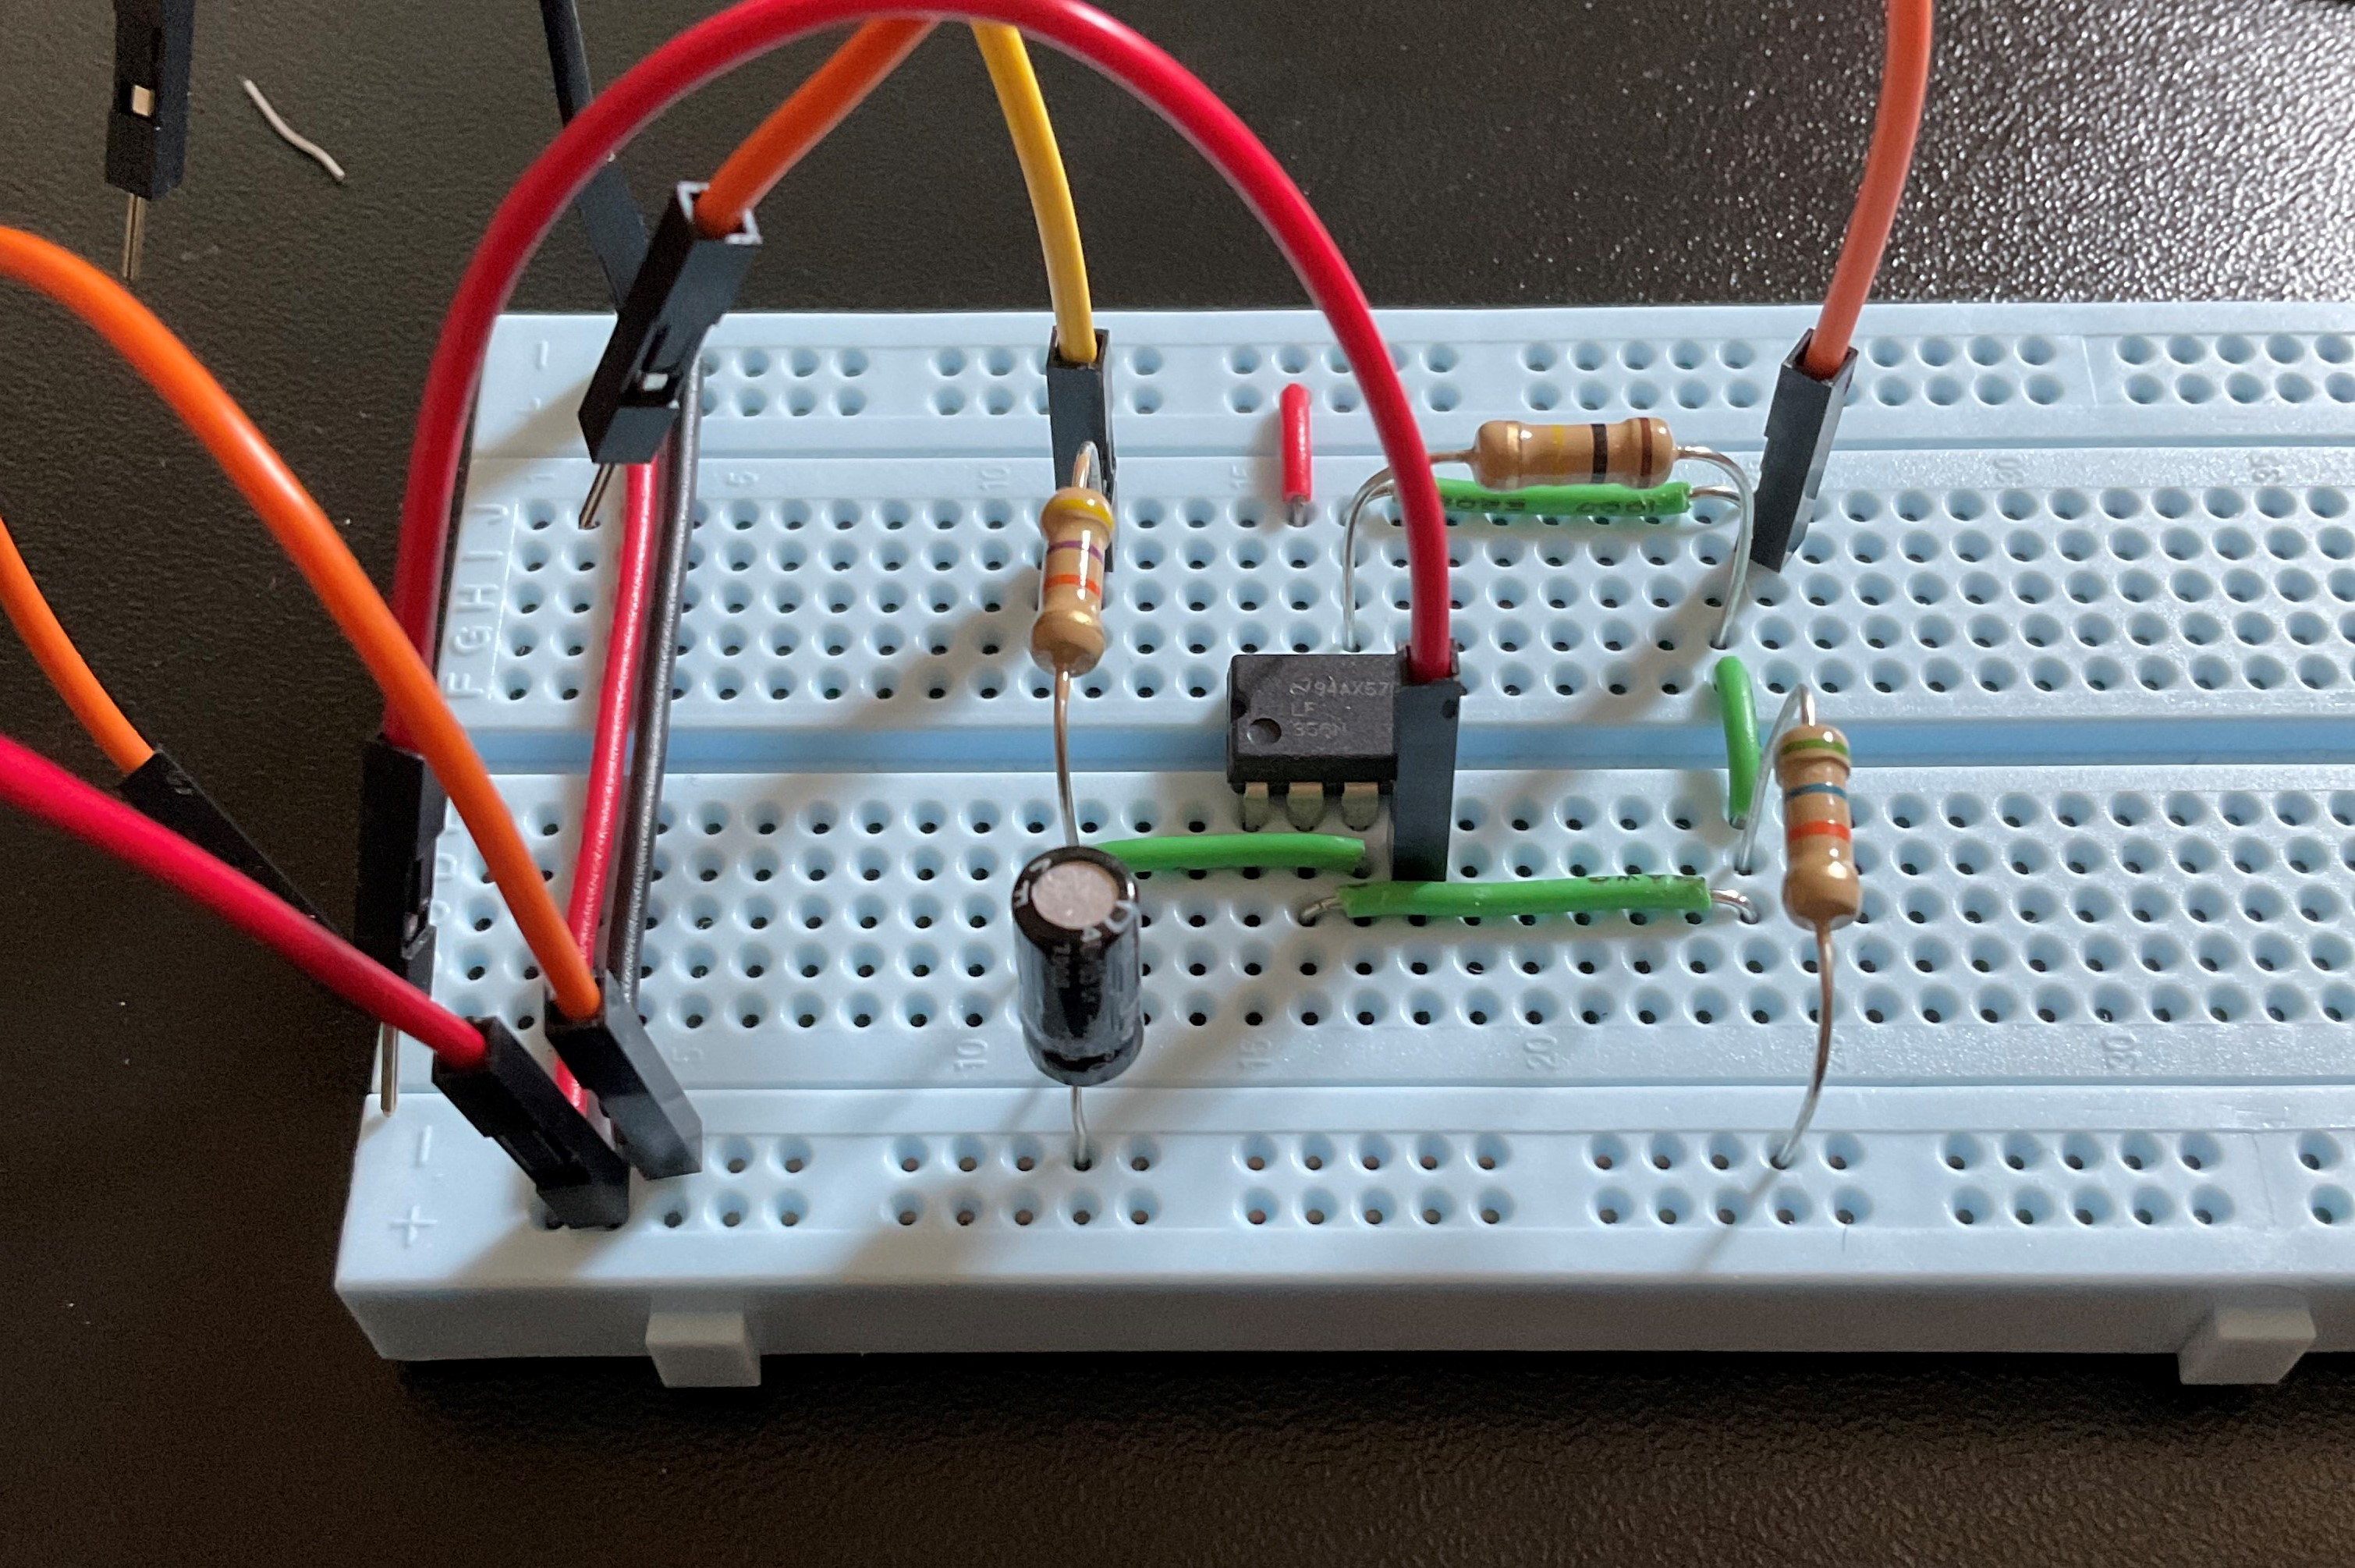
\includegraphics[width = .5\textwidth]{realfilter.jpg}}
\end{center}
Now that we have the real circuit constructed, using the oscilloscope and the wave form we can get the bode plot for the filter circuit.

From the bode plot we can see that the circuit is certainly filtering out the higher frequencies, \textbf{the range of the bode plot is a bit smaller since the data cannot be acquired nearly as quickly} as with the simulation as the trials actually need to occur at real time so for lower frequencies the trials can take upwards of an hour.
\begin{center}
    \boxed{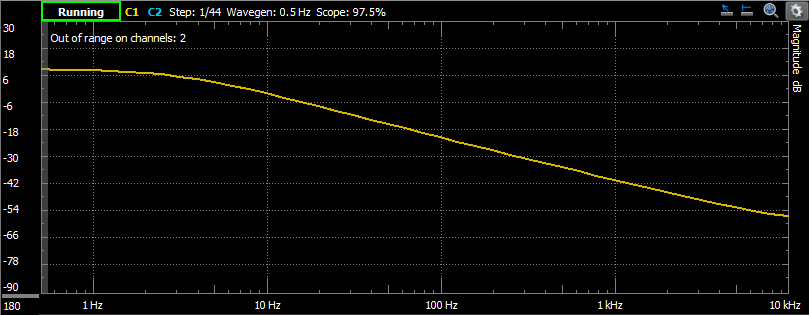
\includegraphics[width = .9\textwidth]{realbode.png}}
\end{center}
Now we have a working filter with an input and output in an easily accessible place.
\end{document}
